\begin{frame}{\expv}
	\textbf{motivation:}
	\begin{itemize} % just present most interesting results here!
		\item stepping from character level to word level
		\item starting point: correlations between activations of an LSTM for formal language phenomena (hierarchy markers BRACE and BRACE)
		\item what kind of information about natural language is learnt by a neural network? (purely sequential vs. hierarchichal information)
		\item which network type (simple recurrent, GRU, LSTM) performs best % this basically should be a comparison to old research AND should facilitate further experiments by knowing what to focus on
		\item this experiment is addressing all presented research questions		
	\end{itemize}
\end{frame}
\begin{frame}{\expv}
	\textbf{procedure:}
	\begin{itemize}
		\item training data: \hdt~part A -- C
		\item test data: a 7000-sentences subset of \hdt~part A
		\item train several neural networks with different architectures, i. e. all three mentioned types with dimensions (512, 512) 
		\item to get a first idea which model is “most qualified“ compute perplexities of language models
		\item look at sentences containing dependency relation DET including a \textit{distractor noun} between the determiner and the real head-noun
		\item mark the sequence from determiner to distractor noun on the one hand and the sequence from determiner to head noun on the other hand % provide an example of marking procedure here, WHY did we choose this particular relation? -> explain
		\item correlate the activations with both markings for each sentence and average over all
	\end{itemize}
\end{frame}
\begin{frame}{\expv}
	\textbf{results:}
	\begin{table}
		\centering
		\begin{tabular}{c|c|c||c}
			simple recurrent & GRU & LSTM & trigram (Laplace)\\
			\hline \\
			7500 & 3300 & 2500 & 26000
		\end{tabular}
		\caption{Approximate perplexity values of networks}
	\end{table}
\end{frame}
\begin{frame}{\expv}
\textbf{some examples:}
\begin{itemize}

\item \textit{der die diz über die säule sind dennoch vage nach eigenen angaben von office auf 351 umzusteigen}

\item \textit{dort in peking und athlon-mainboards}

\item \textit{aus für arbeit}
\end{itemize}

\end{frame}
\begin{frame}{\expv}
	\begin{itemize}
		\item low average correlations, but for each sentence stronger correlations up to \texttt{0.8}
	\end{itemize}
\end{frame}
\begin{frame}{\expv}
	\begin{figure}
		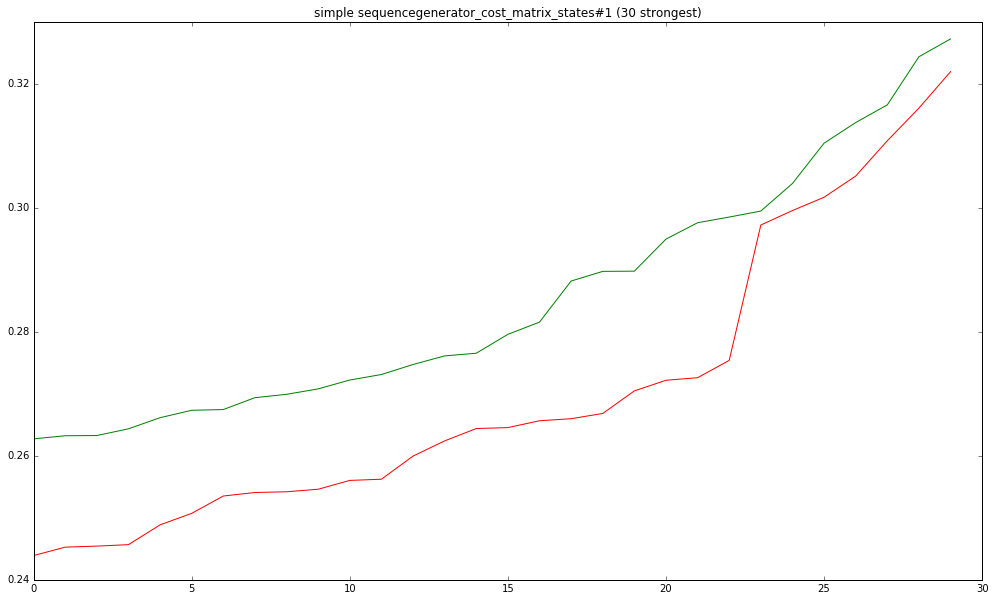
\includegraphics[width=250pt,height=150pt]{gfx/simplernn.png}
		\caption{simple recurrent, last hidden layer output (top 30 correlations)}
	\end{figure}
\end{frame}
\begin{frame}{\expv}
	\begin{figure}
		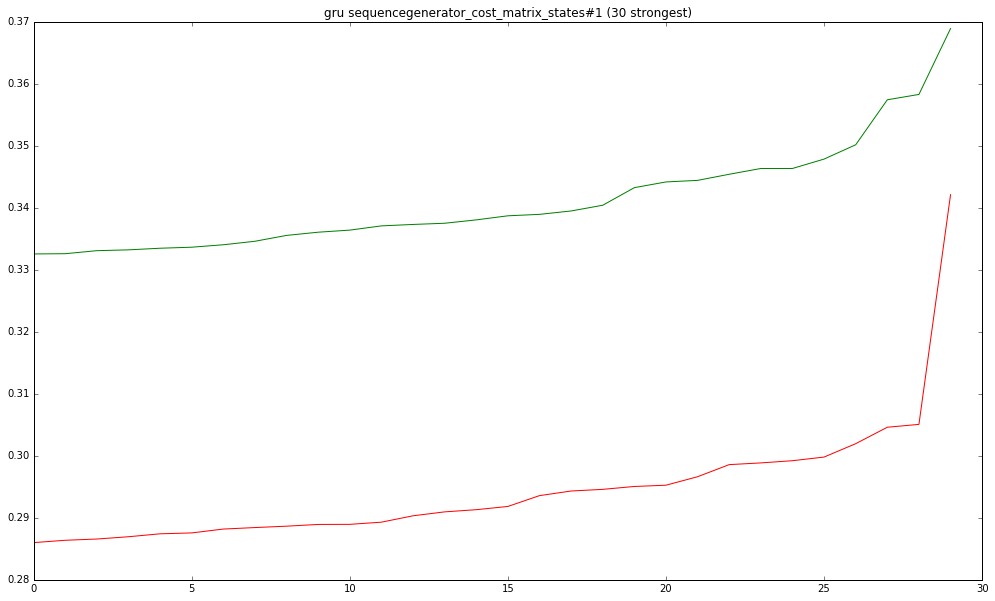
\includegraphics[width=250pt,height=150pt]{gfx/gru.png}
		\caption{gru, last hidden layer output (top 30 correlations)}
	\end{figure}
\end{frame}
\begin{frame}{\expv}
	\begin{figure}
		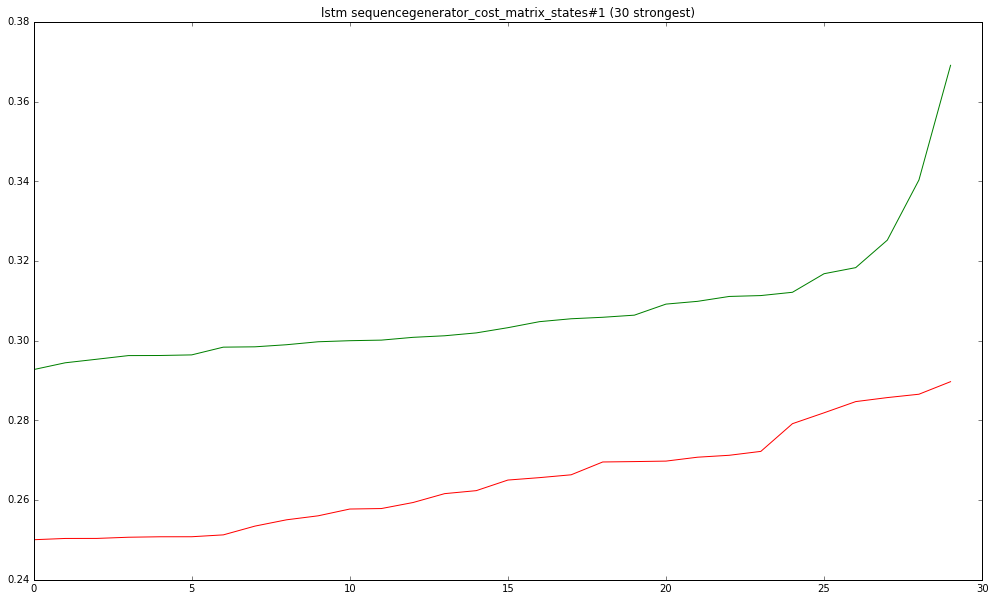
\includegraphics[width=250pt,height=150pt]{gfx/lstmstates.png}
		\caption{lstm, last hidden layer states output (top 30 correlations)}
	\end{figure}
\end{frame}
\begin{frame}{\expv}
\begin{figure}
	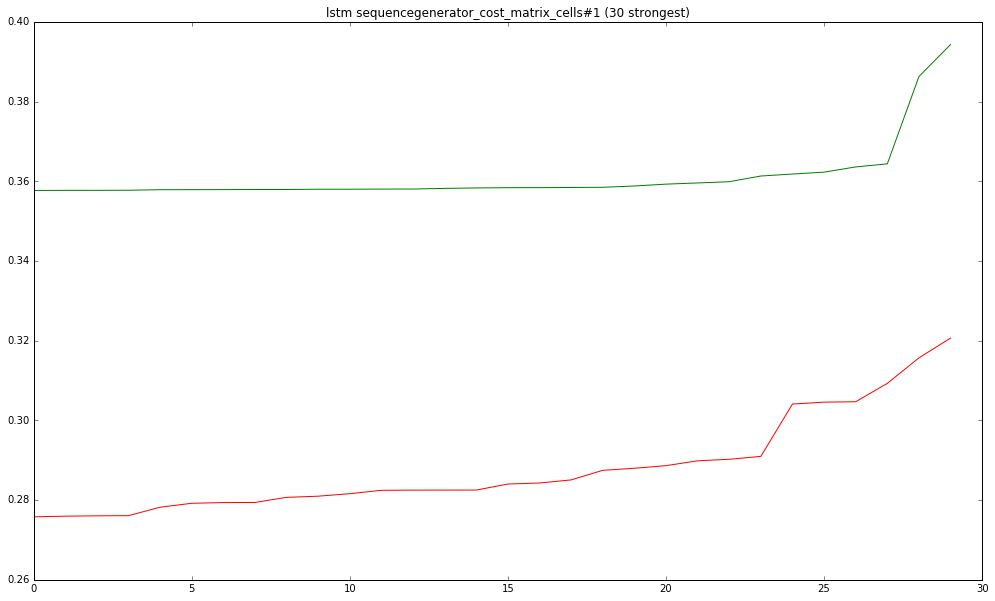
\includegraphics[width=250pt,height=150pt]{gfx/lstm.png}
	\caption{lstm, last hidden layer cells output (top 30 correlations)}
\end{figure}
\end{frame}
\begin{frame}{\expv}
	\textbf{conclusion:}
	\begin{itemize}
		\item no consistent behaviour of a single neuron over all sequences, but strong correlations of single neurons over a subset of the tested sentences
		\item do neurons \textit{cooperate} or \textit{share tasks}
		\item very unclear if these results truly represent a correlation with our phenomenon of choice
	\end{itemize}
\end{frame}